\section{Introduction} \label{int}
Predictability is a defining feature of the rule of law~\cite{frost2015predictability}. Simply put, the outcome of a case should be reasonably predictable based on the legal rules and the facts of the case. Within the field of Legal Judgment Prediction, prison term prediction (PTP) has emerged as a growing yet challenging area~\cite{kim-2014-convolutional,DBLP:conf/ijcai/FengL022,DBLP:journals/access/CuiSW23,zhong-etal-2020-nlp}.
% As a fundamental principle in legal systems, \textit{foreseeability} emphasizes the clarity and predictability in laws~\cite{a072cee8, doi:10.1086/467670}. 
%Foreseeability ensures that individuals can anticipate the legal consequences of their actions, particularly in the context of violating the law~\cite{a072cee8, doi:10.1086/467670}. 
% Imprisonment Term Prediction (PTP) methods embody this principle by predicting the legal consequences based on individuals' actions, ensuring the judicial decisions align with legal standards~\cite{doi:10.1080}. 
%Additionally, Imprisonment Term Prediction (PTP) tools can assist in screening judicial decisions to ensure their alignment with legal standards.
% Such technological advancements not only reflect the capacity to foresee legal outcomes but also serve as a warning to individuals who intend to conduct unlawful activities. 
% PTP has long been a challenge in legal judgment prediction~\cite{DBLP:conf/ijcai/FengL022,DBLP:journals/access/CuiSW23,zhong-etal-2020-nlp}. 

Most existing studies on PTP solely focus on understanding the current case content and historical cases to predict judicial outcomes.~\cite{devlin-etal-2019-bert,DBLP:conf/iclr/ClarkLLM20,Rformer,DBLP:conf/cicai/ZhouLWKZW22}. 
% Consequently, these methods fail to harness the inherent legal knowledge found in law articles, limiting their ability to infer judicial outcomes according to legal principles.
As a result, these methods do not fully utilize the knowledge embedded in legal rules, thereby limiting their accuracy in predicting prison terms.
Recent research has sought to integrate legal knowledge in legal rules into PTP~\cite{neurjudge,ML-LJP}. Nevertheless, these methods represent legal rules as plain texts, overlooking the intrinsic structure of legal rules.
% that embodies the legal decision-making process. 
Effective representation of the \emph{structural information} embedded in legal rules remains an ongoing challenge.

\begin{figure}[!t]
    \centering
    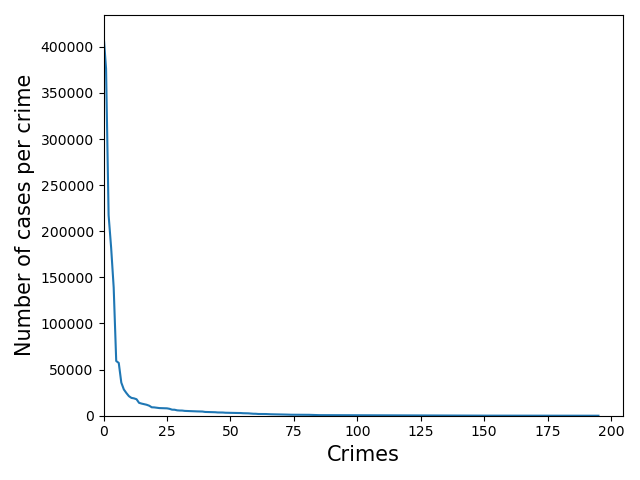
\includegraphics[width=0.9\columnwidth]{figs/sta2.png}
    \caption{Distribution of cases per crime in CAIL2018~\cite{DBLP:journals/corr/abs-1807-02478}. 
    % It shows that nearly 50 crimes are less than 100 cases.
    % \KZ{I still don't understand this graph. Should it be num of cases per crime type? You wanna show many crimes have just a small number of cases?} 
    }
    \label{fig:sta}
    \vspace{-1.5em}
\end{figure}

Another challenge facing current PTP research is the \textit{limited availability of training data for many criminal charges}, as depicted in Figure~\ref{fig:sta}. It shows that nearly 50 crimes are less than 100 cases.
% Another challenge in PTP is the \emph{scarcity of training data for most charges}, as depicted in \figref{fig:sta}. 
Furthermore, legal terms may vary in interpretation across different statutory provisions. For instance, in Chinese law, ``Large Amount'' refers to amounts exceeding 1,000 and 100,000 yuan in the charges of ``Crimes of Theft'' and ``fundraising fraud'', respectively; ``Serious Circumstance'' denotes repeated thefts and illegal operations exceeding 200,000 yuan in the charges of ``Crimes of Theft'' and ``Copyright Infringement'', respectively. 
The state-of-the-art PTP methods~\cite{neurjudge,ML-LJP} are built upon pre-trained language models~\cite{devlin-etal-2019-bert}. Due to the scarcity of cases per crime, 
% \KZ{the meaning of ``per charge'' is not clear. What we want to express is a ``kind'' of criminal violation. Later on you talked about ``Crime of Load Fraud''. So instead of charge, shall we say ``crime''? You need to set the terminology straight first.} 
fine-tuning language models specifically for each crime proves challenging for these methods. Consequently, these models are often trained on judgments of all crimes, hindering their ability to capture the differences in the meanings of certain legal terms in different crimes.

% Meanwhile, with the prevalence of pre-trained language models and Large Language Models (LLMs), recent research has delved into their potential to enhance PTP performance~\cite{}. Since these models are not tailored specifically to law articles and legal case documents, they require fine-tuning on law datasets. Nevertheless, very few case documents are available for most crime types in criminal law, as illustrated in Fig.~\ref{fig:sta}. This often results in insufficient documents for fine-tuning these pre-trained language models and LLMs regarding a specific crime type. Conversely, fine-tuning pre-trained models on documents of all types fails to capture the discrepancies among crime types. This is because the same phrase may correspond to distinct definitions in different crime types, such as \textit{Large Amount} and \textit{Serious Circumstances} in Chinese criminal law. 

%However, there exists a gap between research and real-world applications due to the following issues. 

% \textbf{Misaligned Problem Formulation}. Most previous works model PTP task as a classification problem~\cite{feng-etal-2022-legal,ML-LJP}, merely predicting prison time on a coarse level. These works does not align correclty with the judicial process, where the penalty term is related to the crime type and unlawful action. In terms of severity, there are non-trivial gap between one and six months, and between ten and fifteen years. More importantly, the classification problem setting violates the principle of \textit{lex talionis} (also known as the proportionality principle), which mandates that punishments should be appropriately matched to the nature of the offence, avoiding any discrepancy in severity~\cite{https://doi.org/10.1111/}. 

% \textbf{Sub-optimal Performance}. Previous works studying the PTP task~\cite{wu-etal-2023-precedent,lyu-etal-2023-multi,gan-etal-2023-exploiting} indicate that over half of the cases are incorrectly predicted. Further, when considering their low Macro F1, the outcome is much worse in charges with few cases. Despite some efforts to introduce legal knowledge into models~\cite{neurjudge,ML-LJP}, the result is still not ideal. This indicates an urgent need of more accurate methods towards PTP task.
  


% \begin{table}[]
%     \centering
%     \scriptsize
    
%     \caption{Example of the complexity of statuary provisions. The frequency denotes how many times of legal terms exist in the China Criminal Act of China.}
%     \begin{tabular}{p{0.15\columnwidth}p{0.1\columnwidth}p{0.6\columnwidth}}
%     \toprule
%        Legal Terms  &  Frequency & Example\\
%        \hline
%        Large Amount & 23\% & \emph{''the \underline{amount involved is large} be sentenced to fixed-term imprisonment of not more than five years''} from Article 193\\
%        Huge Amount & 25\% & \multirow{2}{0.6\columnwidth}{\emph{''Where the \underline{amount is huge} or there are other \underline{serious circumstances}, fixed-term imprisonment of no less than five years but no more than ten years shall be imposed concurrently''} from Article 204}\\
%        \addlinespace
%        Serious circumstances & 44\% & \\
%        \bottomrule
%     \end{tabular}
%     \label{tab:words}
%     \vspace{-2em}
% \end{table}

% \textbf{Mixed Crime Types}. Current PTP studies often mix different crime types~\cite{wu-etal-2022-towards}. It is hard for models to capture the discrepancy among mixed charges. The context meaning of the same phrase varies among different different crime types. As highly frequent words in Chinese Criminal Law, for example, \textit{Large Amount} and \textit{Serious Circumstances} have various definitions across different charges. This explains why judges usually specialize in a category of cases. A judge concentrating on injury cases may not have as much domain knowledge as other types. Following the judicial process, predictions should be specific to certain crime types. 

% \textbf{Imbalance and Scarcity in Dataset.} Figure~\ref{fig:sta} presents the statistical results of a well-known LJP dataset named CAIL2018. This dataset is collected from China Judgement Online including at least millions of cases~\cite{DBLP:journals/corr/abs-1807-02478}. The crime types are so imbalanced that over half the crime types have fewer than 1000 cases. Trained on this dataset, the model has an inherent bias towards these frequent crimes and tends to miss those relatively rare ones~\cite{zhong-etal-2020-nlp}.

% \begin{table}[]
%     \centering
%     \small
%     \caption{Representative previous results of Imprisonment Term Prediction. MaF denotes the Macro F1. Results are collected from~\cite{ML-LJP}.}
%     \begin{tabular}{c|cc}
%     \hline
%     \hline
%         Model & Accuracy & MaF \\
%         \hline
%         CNN~\cite{kim-2014-convolutional} & 31.14 & 32.94\\
%         BERT~\cite{devlin-etal-2019-bert} & 41.83 & 41.65\\
%         Electra~\cite{DBLP:conf/iclr/ClarkLLM20} & 42.56 & 41.84\\
%         Neurjudge~\cite{neurjudge} & 37.12 & 36.00\\
%         R-Former~\cite{Rformer} & 43.62 & 43.17\\
%         ML-LJP~\cite{ML-LJP} & 47.63 & 43.17\\
%         \hline
%         \hline
%     \end{tabular}
%     \label{tab:pre}
% \end{table}

To tackle the challenges above, inspired by the graph structure having better representation ability for plain text~\cite{card1999readings,wang-etal-2022-d2gclf,gao-etal-2023-dialogue}, we propose a novel approach to representing statutory provisions in criminal law by \emph{\lawgraph{s}}. A \lawgraph{} encompasses \textit{illegal conducts}, \textit{severity classes}, \textit{judicial outcomes}, and their interconnections, all of which are crucial in determining the prison term of a case. We show that \lawgraph{s} can be accurately constructed from statutory provisions using a rule-based method, capitalizing on the conventional writing style used in drafting statutory provisions. To leverage \lawgraph{s} in PTP, we propose a lightweight \underline{S}tatute \underline{K}nowledge \underline{E}ncoder (SKE) that can be effectively trained on a limited number of judgments. SKE employs a message-passing mechanism tailored for \lawgraph{s} to acquire latent representations that preserve the inherent structural knowledge in the graphs. Then, we utilize the latent representations to match the case facts for prison term prediction. 

Our contributions can be summarized as follows: (1) We identify two critical challenges in prison term prediction, i.e., the structural representation of statutory provisions and the scarcity of training data for individual crimes; (2) We propose \lawgraph, a novel representation of legal rules, and a rule-based approach for parsing statutory provisions into \lawgraph{s}; (3) Leveraging \lawgraph{s}, our method reduces Root Mean Square Error (RMSE) by up to 20.75\% and improves Macro F1 by up to 20\%, compared to the state-of-the-art methods.
%on real-world judgment datasets.
% \begin{enumerate}
% \item 
% \item 
% %We propose a Statute Knowledge Encoder to obtain latent representations of \lawgraph{s} and leverage these representations for prison term prediction. In this way, our solution makes predictions by implicitly referring to legal knowledge inherent in \lawgraph{s}. 
% \item  
% \end{enumerate}

% we propose a new problem: Realistic Imprisonment Term Prediction (RPTP). Unlike PTP, RPTP is a regression problem, aiming to concretely predict imprisonment terms from legal contexts. Moreover, the RPTP framework challenges the process of learning predictive regulations from past cases due to the scarcity of training data. To address this challenge, we propose the Statute Knowledge Enhanced (SKE) method, aimed at compensating for the inadequacies associated with limited training data by enabling the model to derive more comprehensive insights from statutory laws. 

% Our contributions are listed as the following: (1). We conclude four groups of issues from previous works on Imprisonment Term Prediction (PTP). Towards these issues, we propose a new problem: Realistic Imprisonment Term Prediction (RPTP), where the model needs to accurately predict the imprisonment term. (2). We propose our approach, Statute Knowledge Enhanced (SKE), to solve the RPTP problem. SKE incorporate knowledge from statutory laws for penalty term prediction. We propose Law-Graph to better represent legal knowledge. Generally, with multiple edge types and relation types. (3). We conduct comprehensive experiments to compare the performance of SKE with previous works. The results show that SKE outperforms the state-of-the-art works by up to 1, 2, 20\%, and 40\% in terms of Mean Absolute Error (MAE), Root Mean Square Error (RMSE), Macro F1, and Pearson, respectively. (4) We apply Large Language Models (LLMs) to RPTP task and further assess the capabilities of LLMs. The experimental results show that SKE outperform ChatGPT-3.5 and achieve comparable results to ChatGPT-4.

% \begin{enumerate}
% % \vspace{-1em}
% \item We conclude four groups of issues from previous works on Imprisonment Term Prediction (PTP). Towards these issues, we propose a new problem: Realistic Imprisonment Term Prediction (RPTP), where the model needs to accurately predict the imprisonment term.

% \item We propose our approach, Statute Knowledge Enhanced (SKE), to solve the RPTP problem. SKE incorporate knowledge from statutory laws for penalty term prediction. We propose Law-Graph to better represent legal knowledge. Generally, with multiple edge types and relation types.

% \item We conduct comprehensive experiments to compare the performance of SKE with previous works. The results show that SKE outperforms the state-of-the-art works by up to 1\%, 1\%, and 1\% in terms of Mean Absolute Error (MAE), Root Mean Square Error (RMSE) and Macro F1, respectively.

% \item We apply Large Language Models (LLMs) to RPTP task and further assess the capabilities of LLMs. The experimental results show that SKE outperform ChatGPT-3.5 and achieve comparable results to ChatGPT-4.
% \end{enumerate}

